\chapter{LFO}
\label{ch:LFO}

\section{Allgemeines}
Wie bereits in Kapitel \label{ch:concept} beschrieben, wird der LFO genutzt, um niederfrequente Signale zu erzeugen. 
Diese Signale werden typischerweise zur Steuerung von nachgelagerten Modulen, wie etwa dem LFO (siehe Kapitel \ref{ch:VCO}), verwendet.
Hierdurch kann beispielsweise die Frequenz des VCO angepasst werden. 
Neben der Frequenz, die der LFO ausgibt, ist auch die entsprechende Signalform für den Klang entscheidend. Hier sind beispielsweise Signalformen, wie Dreieck oder Rechteck möglich.

\section{Schaltplan}

Im Folgenden wird näher auf den Schaltplan des LFO eingegangen, welcher in Abbildung \ref{fig:LFO_Stromlaufplan} zu sehen ist \cite{lfo_manual}. 
Ein Bauteil von zentraler Bedeutung ist hierbei der Vierfach-Operationsverstärker TL074P. In der gezeigten Schaltung wird dieser als Integrator, Schmitt Trigger, Buffer und LED-Treiber verwendet.
Die grundlegende Funktionsweise dieser Funktionsgruppen wird in Abschnitt \ref{ch:VCO} erläutert. Aus diesem Grund wird nicht weiter auf die Funktionsweise eines Oszillators eingegangen.

\newpage
\begin{figure}[h]
\centering
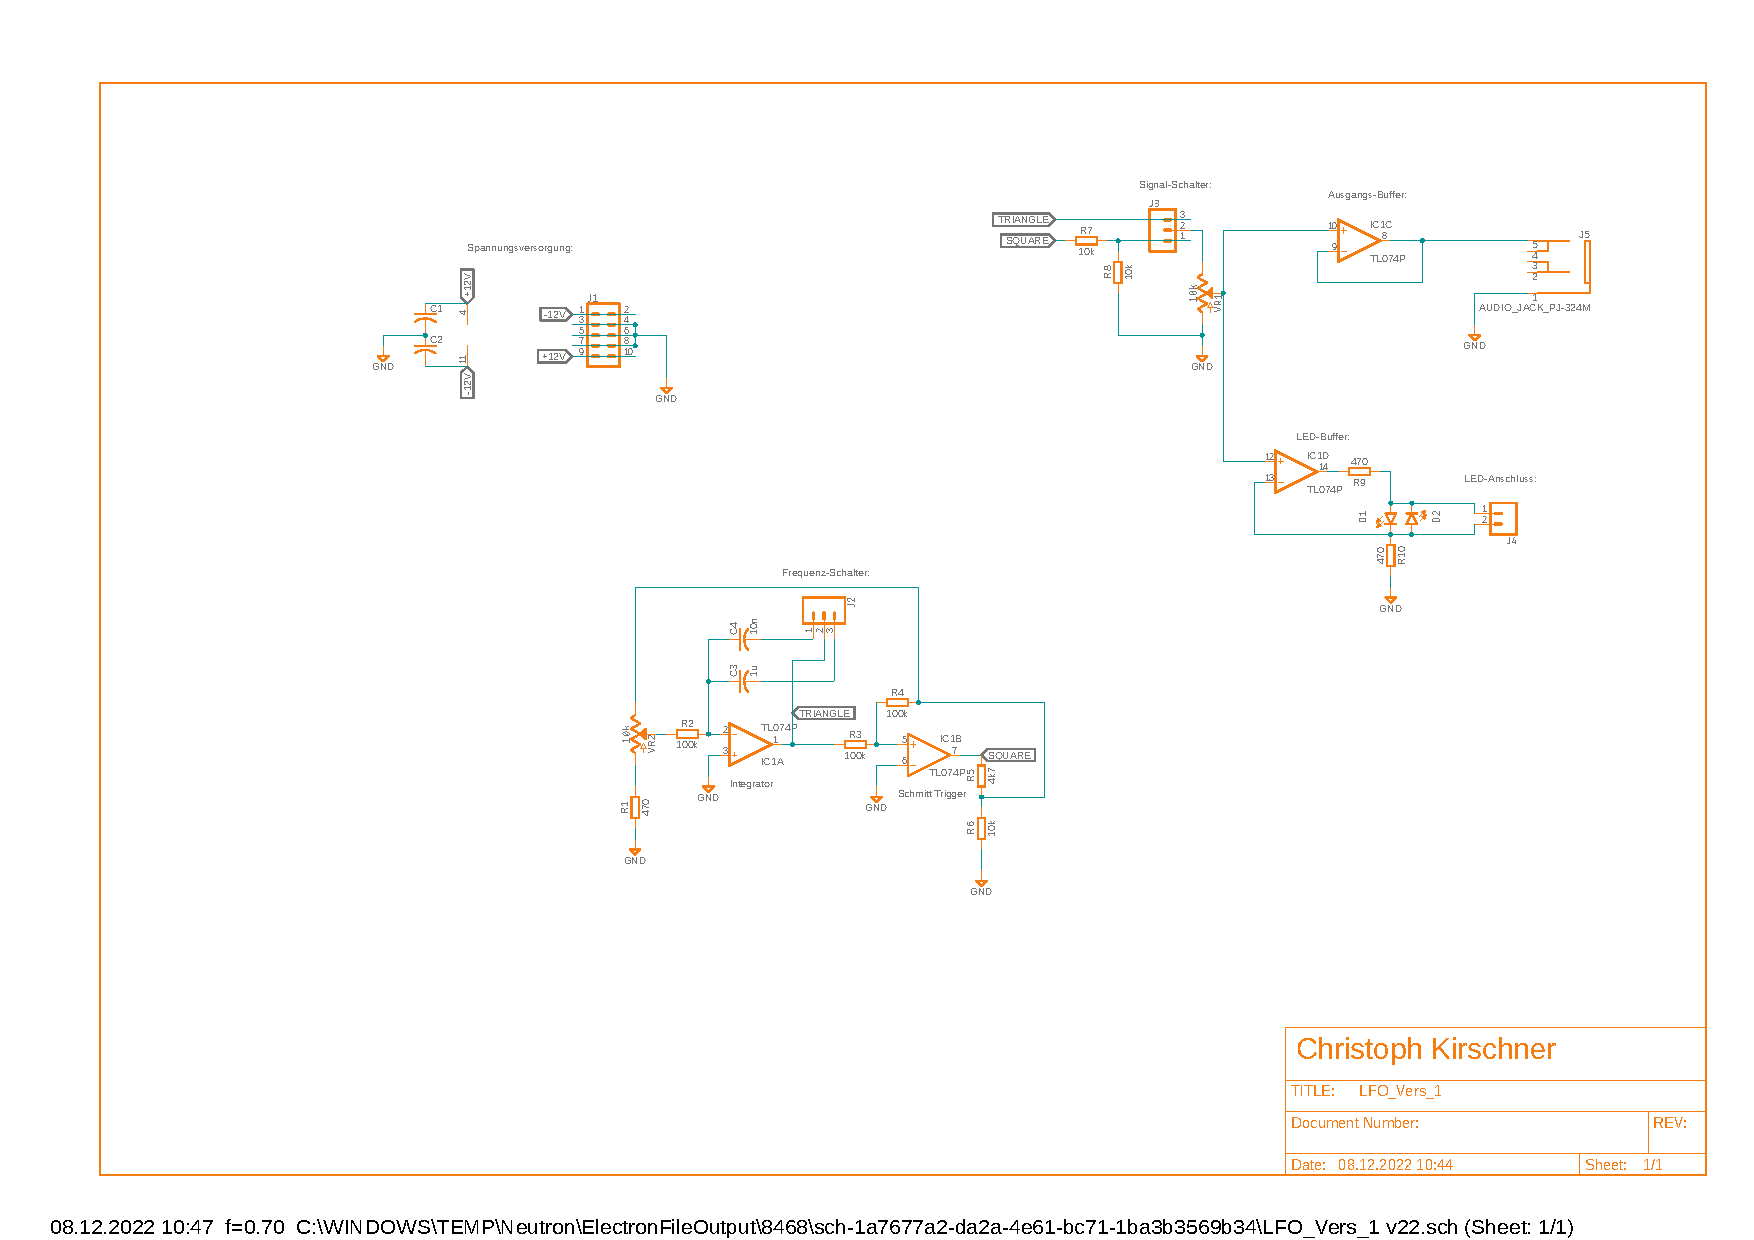
\includepdf[angle=270, clip, trim=1cm 0.8cm 0.8cm 0.8cm, scale=0.8] {figures/Schaltplan_LFO_Kirschner_08_12_22.pdf}
\caption{Fusion360 Schaltplan des LFO}
\label{fig:LFO_Stromlaufplan}
\end{figure}
\FloatBarrier
 
\newpage

\section{Platine}

In Abbildung \ref{fig:PCB_LFO_bottom} ist die untere Lage der Leiterplatte in blau dargestellt. 
Beim Erstellen der Platine wurde der Fokus auf die Produzierbarkeit mittels CNC-Fräße gelegt. 
Hierbei ist die Lagenzahl der Platine auf maximal  zwei Lagen begrenzt, wobei nur einlagiges Platinenrohmaterial zur Verfügung stand. 
Um diese Limitation zu umgehen wurde versucht alle Leiterbahnen auf eine Platinen-Lage zu entflechten. 
Da manche Leiterbahnen nicht auf der Unterseite platziert werden konnten, wurden für die restlichen Bahnen auf der Oberseite Verbindungsdrähte verwendet. 
Hierfür wurden jeweils Via-Verbindungen mit größerem Bohrungsdurchmesser vorgesehen.
Der Vorteil dieser Methode ist, dass die Platine ohne Mehraufwand auch professionell produziert werden kann. 
Die beschriebene Vorgehensweise wurde auch bei den übrigen Platinen dieser Projektarbeit angewendet.

\begin{figure}[h]
	\centering
	\setlength{\fboxsep}{1pt} %Abstand der Linien zur Abbildung
	\setlength{\fboxrule}{1pt} %Dicke der Linie
	\fbox{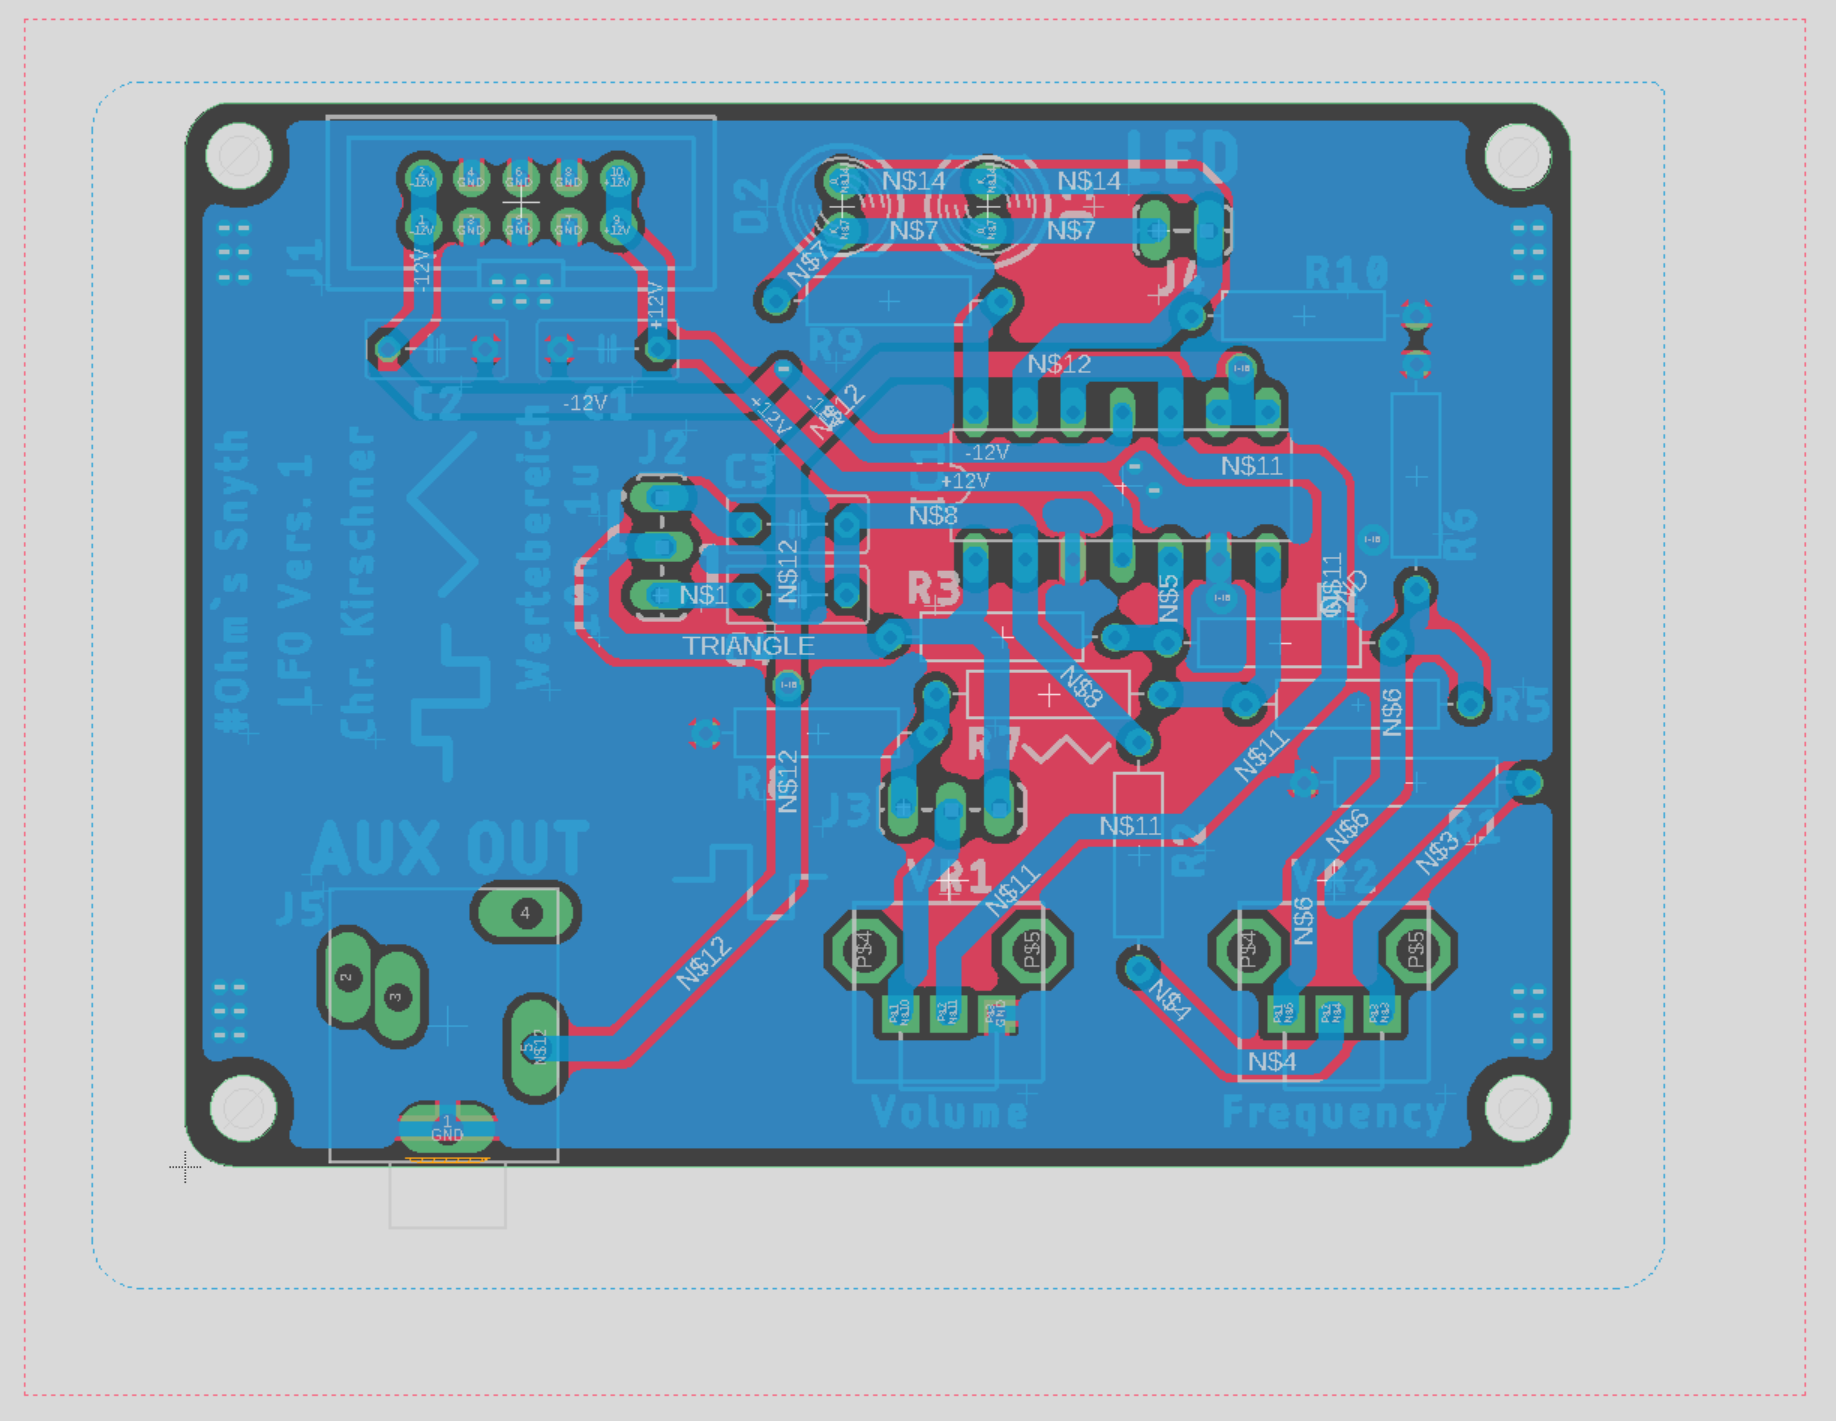
\includegraphics[width=1\textwidth]{figures/Platine_LFO.PNG}}
	\caption{Ausschnitt des LFO-Platinen-Layouts aus Fusion360 (Unterseite)}
	\label{fig:PCB_LFO_bottom}
\end{figure}
\FloatBarrier

\newpage

Wie bereits beschrieben, wurde die Platine mit einer Platinenfräße angefertigt. Hierbei wurde die CNC-Fräße \grqq{}Othermachine\grqq{} von \grqq{}Bantam Tools\grqq{} verwendet. In Abbildung \ref{fig:bantam_tools_lfo} is ein Ausschnitt aus der Steuer-Software von \grqq{}Bantam Tools\grqq{} gezeigt. Mit Hilfe dieser Software können Gerber-Dateien oder brd-Dateien (Eagle) importiert werden und Fräßabläufe erzeugt werden.

\begin{figure}[h]
	\centering
	\setlength{\fboxsep}{1pt} %Abstand der Linien zur Abbildung
	\setlength{\fboxrule}{1pt} %Dicke der Linie
	\fbox{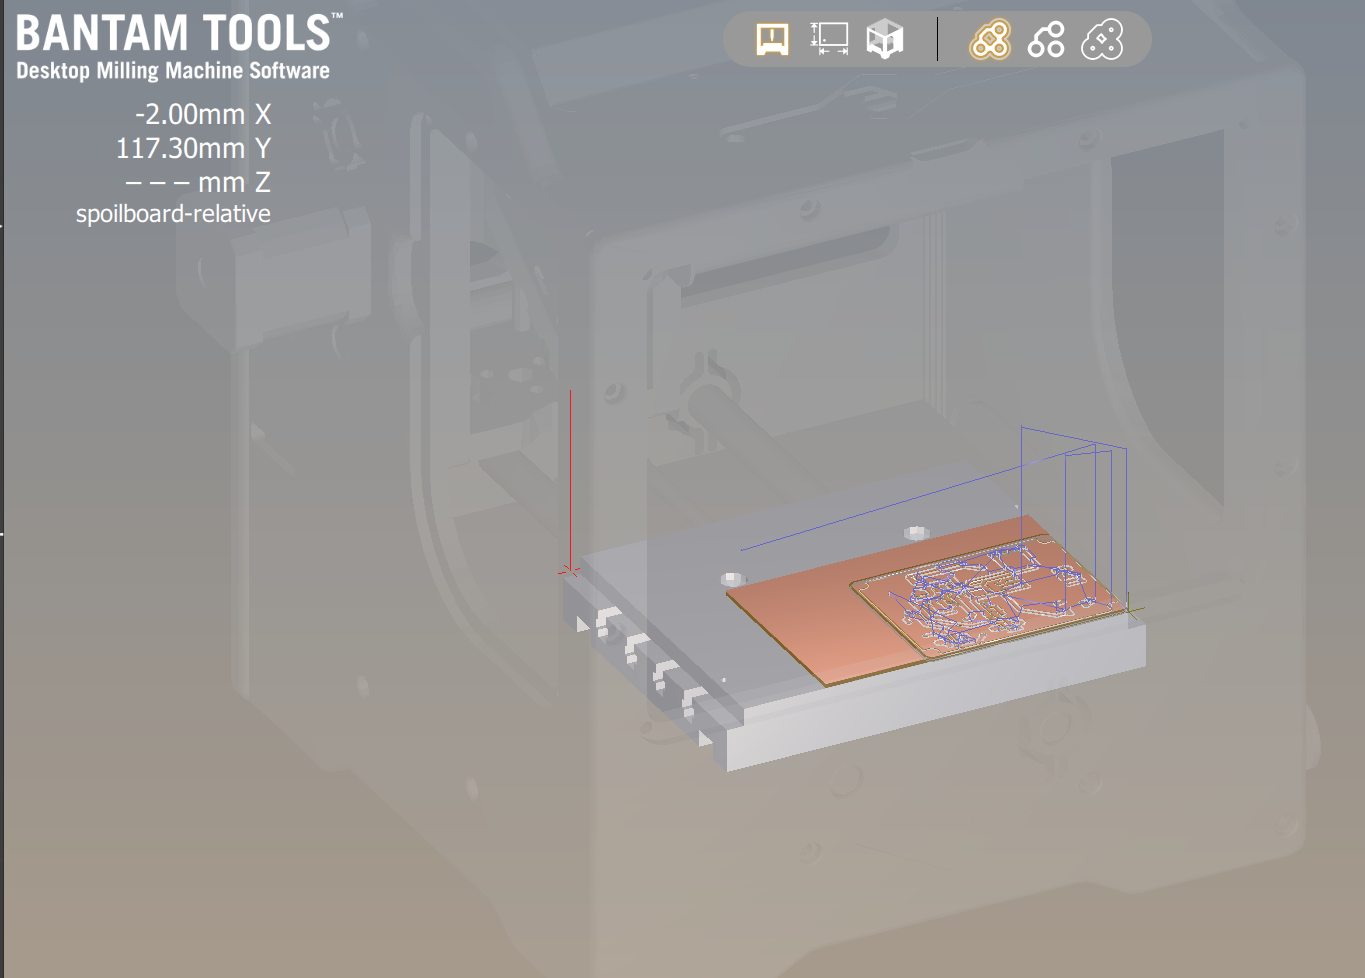
\includegraphics[width=1\textwidth]{figures/Bantam_Tools_LFO.PNG}}
	\caption{3D-Ansicht der LFO-Platine in Bantam-Tools-Software (Platinen-Fräße) \cite{bantam}}
	\label{fig:bantam_tools_lfo}
\end{figure}
\FloatBarrier

\newpage

\section{Mechanischer Aufbau}
Um die LFO-Platine in einem Rack-System befestigen zu können, ist es nötig eine entsprechende Abdeckplatte mit Montagelöchern an der Platine anzubringen. 
Die Befestigung der Frontplatte an der LFO-Platine wird über das Gewinde an der AUX-Buchse realisiert. Dies hat sich bei lediglich einer Buchse als nicht ausreichend herausgestellt. Aus diesem Grund wurde die Platine zusätzlich mit Epoxit-Kleber an der Abdeckplatte fixiert.

\begin{figure}[h]
	\centering
	\setlength{\fboxsep}{1pt} %Abstand der Linien zur Abbildung
	\setlength{\fboxrule}{1pt} %Dicke der Linie
	\fbox{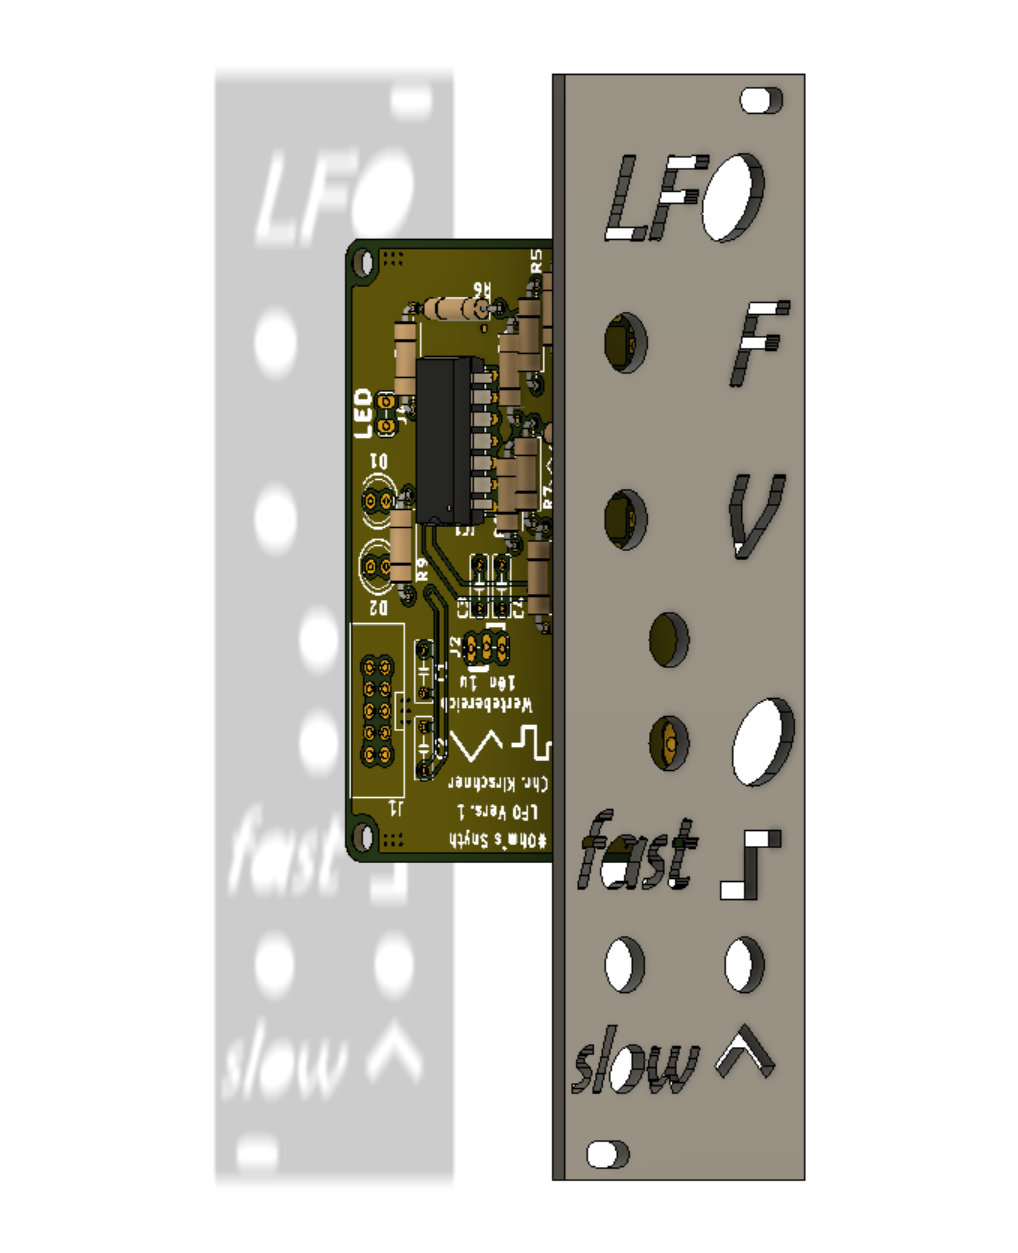
\includegraphics[width=0.6\textwidth]{figures/LFO_Abdeckung_mit_Platine.PNG}}
	\caption{3D-Darstellung der LFO-Platine mit Frontplatte}
	\label{fig:Frontplatte_LFO}
\end{figure}
\FloatBarrier

Wie in \ref{fig:Frontplatte_LFO} abgebildet, wurden die Beschriftungen als Ausschnitte in der Frontplatte angebracht. Hierdurch kann die Frontplatte mit einem Lasercutter kostengünstig produziert werden und es ist somit keine weiter Nachbearbeitung der Frontplatte nötig.

Um bereits vor dem Lasercutten der Frontplatte die grundsätzliche Tauglichkeit der Konstruktion erproben zu können, wurde mittels eines 3D-Drucker die Frontplatte gedruckt. Hierbei wurde ein \grqq{}Prusa Mini\grqq{} und die dazugehörende \grqq{}Prusa Sliver\grqq{}-Software verwendet. Ein Ausschnitt dieser Software ist in Abbildung \ref{fig:3DDruck_LFO} zusehen.

\begin{figure}[h]
	\centering
	\setlength{\fboxsep}{1pt} %Abstand der Linien zur Abbildung
	\setlength{\fboxrule}{1pt} %Dicke der Linie
	\fbox{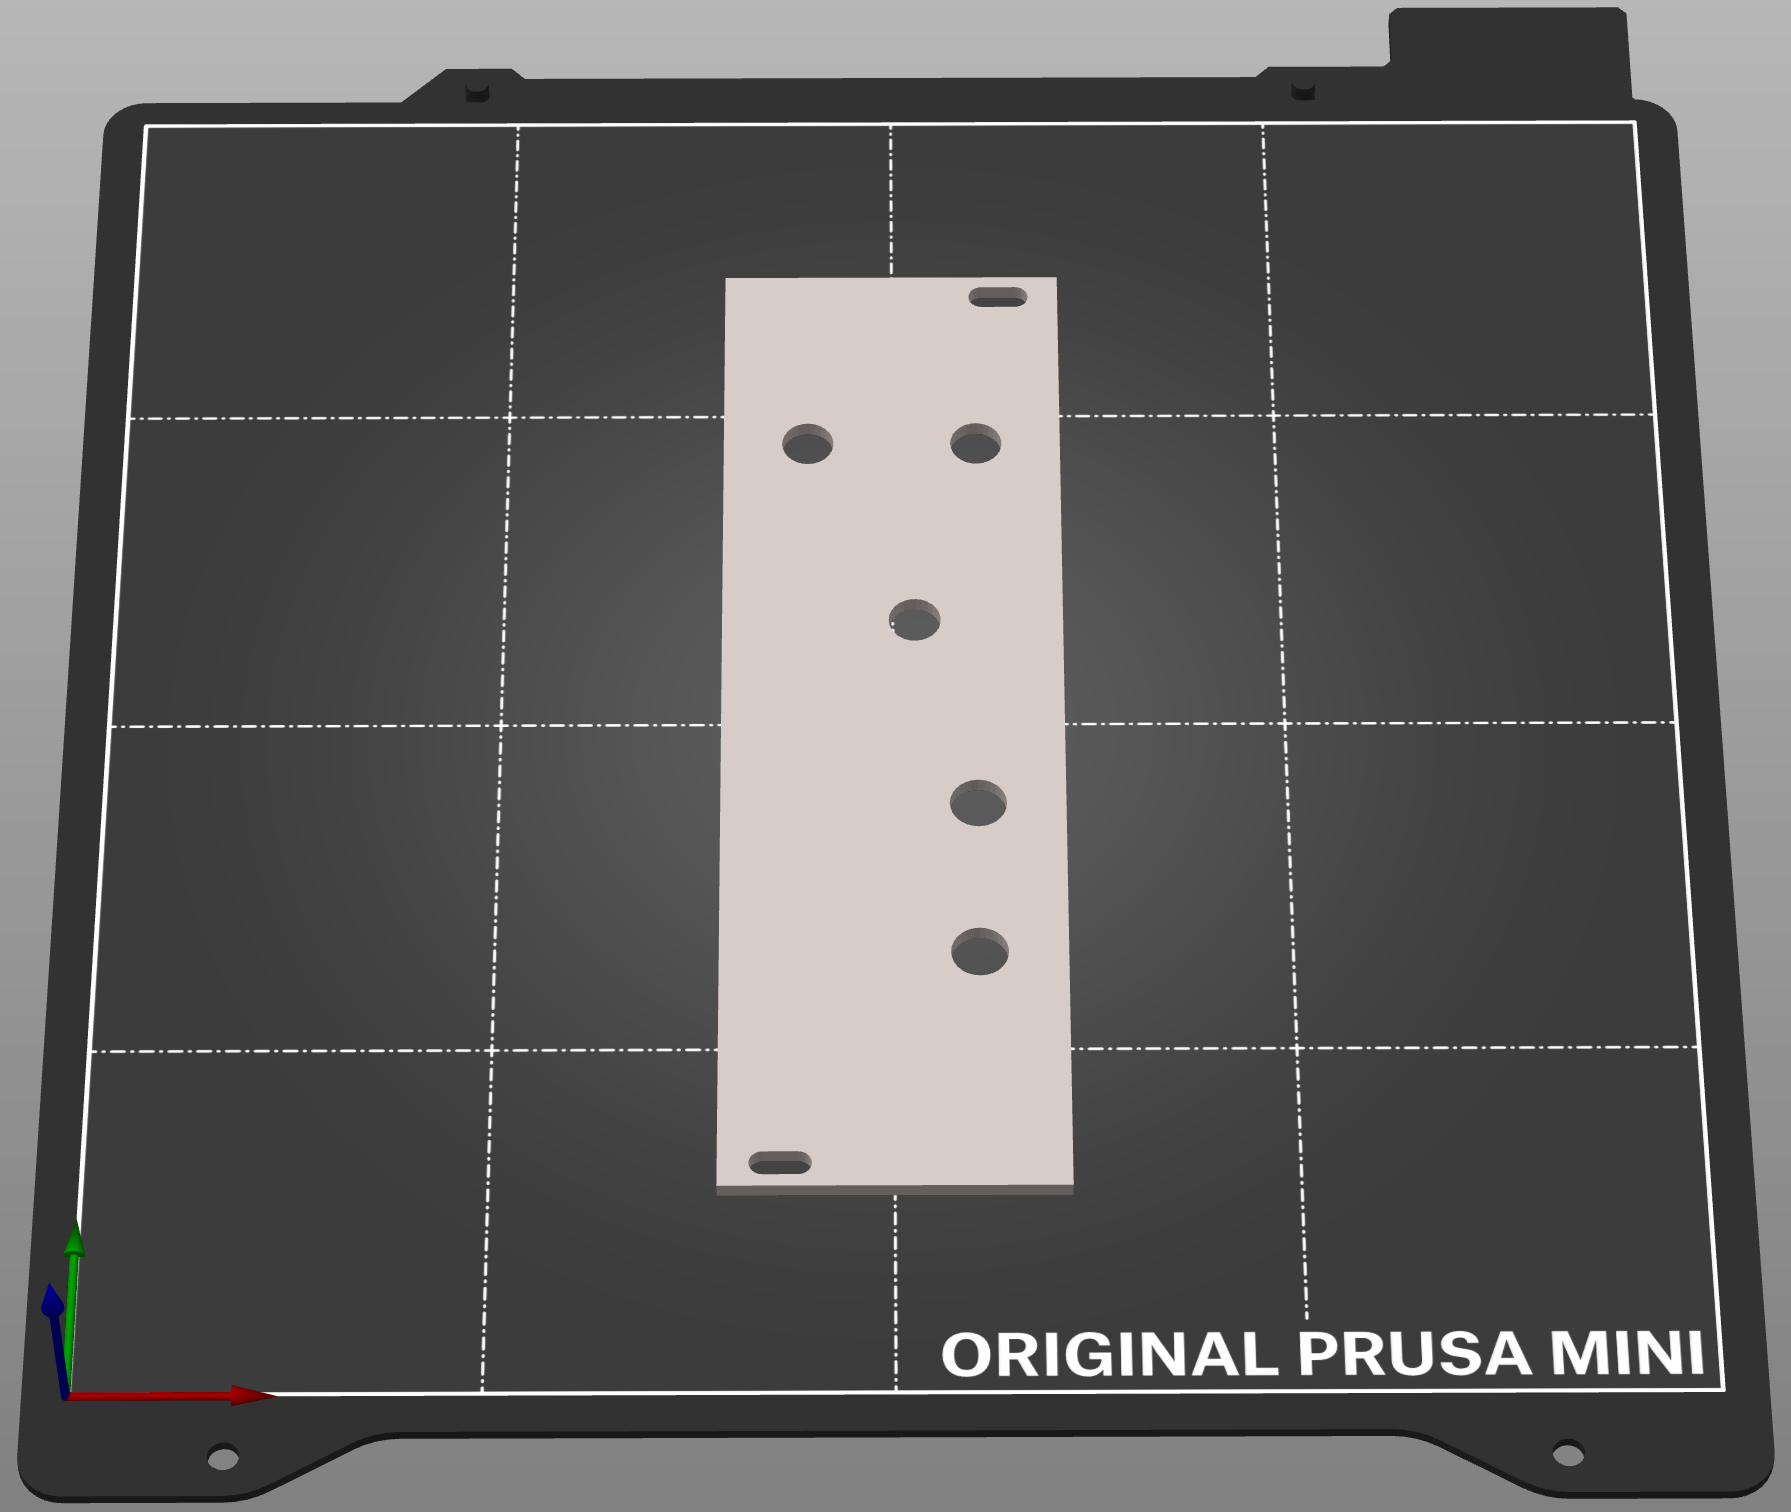
\includegraphics[width=1\textwidth]{figures/Prusa_STL.PNG}}
	\caption{Ausschnitt aus \grqq{}Prusa Slicer\grqq{} beim Vorbereiten des 3D-Drucks für die LFO-Platine \cite{prusa}}
	\label{fig:3DDruck_LFO}
\end{figure}
\FloatBarrier

Die in diesem Abschnitt aufgezeigte Vorgehensweise beim Prototypen der Abdeckplatte ist exemplarisch für alle Module dieser Projektarbeit. Aus diesem Grund wird in den folgenden Kapiteln nicht näher darauf eingegangen.